
\def\g4{{\sf Geant4}}

\newcommand{\codeAlgorithm}[1]{
\addcontentsline{toc}{section}{Résumé}
\begin{center}\fbox{\parbox{12cm}{\bf #1}}\end{center}}

\newcommand{\cppintro}[1]{
\lstset{language=C,
caption= #1 ,
label=listing:boundary}}

\def\cppstart{\begin{lstlisting}}
\def\cppend{\end{lstlisting}}%% Uncomment these if you write in English

\documentclass[12pt]{article}
\usepackage[english]{thesis}

\usepackage[utf8]{inputenc} % look here if scands are broken

%% Jos käytät latex-komentoa käännettäessä (oletusarvo) 
%% kuvat kannattaa tehdä eps-muotoon. Älä käytä ps-muotoisia kuvia!
%% Käytä seuraavaa latex-komennon ja eps-kuvien kanssa 
%%\usepackage[dvips]{graphicx}

%% Jos tääs käytät pdflatex-komentoa, 
%% joka kääntää tekstin suoraan pdf-tiedostoksi ja kuvasi
%% ovat esim. jpg-formaatissa tai pdf-formaatissa,   
%% käytetään seuraavaa pakettia, kommentoi siis kommenttimerkki pois
%% Huom! Tekstin marginaalit saattavat poiketa n. 2-5 mm
%% suosituksesta, jos käytät pdflatex-komentoa!
\usepackage[pdftex]{graphicx} 
\usepackage{multirow}
\usepackage{url}
\usepackage{listings}
%\usepackage{graphicx}
\usepackage[utf8]{inputenc} % look here if scands are broken
\usepackage{wrapfig}
%\usepackage{makeidx}
\usepackage{subfig}
\usepackage{fancyhdr}
%\usepackage{asymptote}
\usepackage{amsmath}
\usepackage{verbatim} % for comment
\usepackage{eurosym} 
\usepackage{color} % for definecolor
\usepackage[colorlinks,bookmarks=true]{hyperref}

%% Saat pdf-tiedoston viittaukset ja linkit kuntoon seuraavalla paketilla.
%% Paketti toimii erityisen hyvin pdflatexin kanssa. 
%\usepackage[pdfpagemode=None,colorlinks=true,urlcolor=red,%
%linkcolor=blue,citecolor=black,pdfstartview=FitH]{hyperref}

%% Jos et jostain syystä tykkää käyttää
%% edellistä hyperref pakettia, voit käyttää myös seuraavaa pakettia
%% (tarvitaan lähinnä url-komennon määrittämiseen ja formatoimiseen)
\usepackage{url}

%% Matematiikan fontteja, symboleja ja muotoiluja lisää, näitä tarvitaan usein 
\usepackage{amsfonts,amssymb,amsbsy}  

%% Käytä seuraavaa pakettia jos haluat
%% Times-fontit LaTeX:n normaalien Computer Modern-fonttien sijaan.
%% Times-fontit ja Computer Modern-fontit ovat kummatkin roomalaisia
%% fonttityyppejä ja monet kutsuvat kaikkia roomalaisia
%% fontteja virheellisesti Times-fonteiksi,
%% vaikka tarkasti ottaen Times on vain Times-lehden fontti.
%% Computer Modern on Donald Knuthin suunnittelema fontti, joka
%% on Century Magazinen fontin variantti.
%% Huom! Kaavoihin ei tule Times-fontteja, joten lopputulos ei ole
%% välttämättä aivan tyylikäs. Pakettia ei suositella sen vuoksi. 
%\usepackage{times}  

%% Vaakasuunnan mitat, ÄLÄ KOSKE!
\setlength{\hoffset}{-1in}
\setlength{\oddsidemargin}{35mm}
\setlength{\evensidemargin}{25mm}
\setlength{\textwidth}{15cm}
%% Pystysuunnan mitat, ÄLÄ KOSKE!
\setlength{\voffset}{-1in}
\setlength{\headsep}{7mm}
\setlength{\headheight}{1em}
\setlength{\topmargin}{25mm-\headheight-\headsep}
\setlength{\textheight}{23cm}
%% Vasensuora-asettelu, joka opinnäytteessä vaaditaan. ÄLÄ KOSKE
\setlength{\parindent}{0pt}
\setlength{\parskip}{1ex}


%% Kaikki mikä paperille tulostuu, on tämän jälkeen
\begin{document}

\Language{English}{Englanti}

\university{helsinki university of technology}{teknillinen korkeakoulu}

%% Korjaa seuraavat vastaamaan omaa tiedekuntaasi
\faculty{Faculty of Information and Natural Sciences}%
{}%
%%

%% Vain kandityölle: Korjaa seuraavat vastaamaan tutkinto-ohjelmaasi
\degreeprogram{Engineering Physics and Mathematics}{}
%%

%% Vain DI- ja lisensiaatintyölle
%\professorship{Circuit theory}{Piiriteoria}
%\code{S-55}
%%

%% Valitse yksi näistä kolmesta
\degree{BSc}
%\degree{MSc}
%\degree{Lic}

%% Oma nimi
\author{Gillis Danielsen}

%% Opinnäytteen nimi tulee vain tähän
\thesistitle{Simulating carbon beam fragmentation on water phantom with the Geant4 INCL/ABLA models}{}

%% Kandidaatintyön päivämäärä on sen esityspäivämäärä! 
%%\date{22.1.2008}

%% Kandidaattiseminaarin vastuuopettaja
\supervisor{Ph.D. Veikko Karimäki, Prof. Harri Ehtamo}{}

%% Kandidaatintyön ohjaaja
\instructor{Aatos Heikkinen}{}

%% Tehdään kansilehti
\makecoverpage

\begin{comment}
\title{Simulating carbon beam fragmentation on water phantom with the Geant4 INCL/ABLA models}

\begin{titlepage}
\pagestyle{empty}
\begin{center}
rev. 001-2009\\
\vspace{7.5 cm}
\Huge
Simulating carbon beam fragmentation on water phantom with the Geant4 INCL and ABLA models\\

\vspace{5cm}

\Large
Gillis Danielsen, Bachelor's Thesis\\
Helsinki University of Technology\\

    \vspace{0,2cm}
  \end{center}

\end{titlepage}
\end{comment}

%% Tiivistelmän avainsanat 
\keywords{Geant4, INCL, Liege cascade, ABLA, CERN, IAEA, Hadrontherapy}
%% Tiivistelmän tekstiosa
\begin{abstractpage}[english]
This paper focuses on the simulation of carbon beams in a water phantom using Geant4 code as a medical application. Geant4 is a multi-purpose physics simulation package developed at CERN, Switzerland. Geant4 currently hosts multiple models suitable for the experiment, however, this paper will focus on the INCL and ABLA models developed as a collaboration of scientists at CERN, GSI, HIP and CEA. Results will be compared to experimental data made available by the GSI Darmstadt/E.Haettner. This work is part of the International Atomic Energy Agency(IAEA) coordinated programme to compile and evaluate charged-particle nuclear data and related Monte-Carlo codes for therapeutic applications. This work introduced extensions to the Geant4 Hadrontherapy-example, using our modelling weestimate particularly the magnitude of fragment build-up at the end of the Bragg-curve.
\end{abstractpage}

%% Pakotetaan uusi sivu varmuuden vuoksi, jotta 
%% mahdollinen suomenkielinen ja englanninkielinen tiivistelmä
%% eivät tule vahingossakaan samalle sivulle
\newpage



%% Sisällysluettelo
%% addcontentsline tekee pdf-tiedostoon viitteen sisällysluetteloa varten
\addcontentsline{toc}{section}{Contents}
%% Tehdään sisällysluettelo
\tableofcontents


%% Symbolit ja lyhenteet
\mysection{Symbols and legends}

\begin{tabular}{ll}
CERN         & Organisation europeenne pour la researche nucleare \\
INCL      & intranuclear cascade, liege\\
ABLA        & Abla \\tion Abration model\\
IAEA         & International Atomic Energy Association \\
HIP        & Helsinki Institute of Physics
\end{tabular}


%% Sivulaskurin viilausta opinnäytteen vaatimusten mukaan:
%% Aloitetaan sivunumerointi arabialaisilla numeroilla (ja jätetään
%% leipätekstin ensimmäinen sivu tyhjäksi, 
%% ks. alla \thispagestyle{empty}).
%% Pakotetaan lisäksi ensimmäinen varsinainen tekstisivu alkamaan 
%% uudelta sivulta clearpage-komennolla. 
%% clearpage on melkein samanlainen kuin newpage, mutta 
%% flushaa myös LaTeX:n floatit 
\cleardoublepage
\storeinipagenumber
\pagenumbering{arabic}
\setcounter{page}{1}


%% Ensimmäinen osa, LEIPÄTEKSTI ALKAA
\section{Introduction}
\thispagestyle{empty}
%Carbon beams are a promising new alternative to traditional radiation cancer therapy. 
The history of radiation treatments dates back to 1895 when W.K.~Roentgen discovered the x-rays. It was not long before these photon rays were used to treat malign tissue. The first methods used were on today's standards very crude, and much work has gone into perfecting the treatments in order to minimize the effect of the rays on the surrounding healthy tissue and maximize the dose delivered to the malign tissue.

However, due to the statistical nature of the photon interactions, a beam of many photons is
exponentially attenuated yielding an exponential decrease of the dose with the depth. To
obtain a higher dose in the tumor than in the surrounding normal tissue, many irradiation
fields are used. The cost of this method is that a large volume of the normal tissue
will suffer from a high dose. By replacing the x-rays with high energy photons, the dose
maximum is shifted a few centimeters deeper and the exponential decrease is more shallow,
which improves the ratio between dose in the tumors and in the normal tissue. Although very sophisticated variations of the photon treatments have been perfected over time, photon therapies still produce considerable harm to the surrounding tissue. 

A much younger and less widely used technology are those of hadron- or heavy-ion based radiotherapies. Hadrons and heavyer-ions are charged particles and therefore interact with tissue in a much different way to photons. The dose-profile contains a much sharper peak due to the primary halting force being electromagnetic interaction. This peak is called the Bragg-peak, and was first discovered by William Henry Bragg in 1903.

The field of hadron treatments was pioneered at the Lawrence Berkeley Laboratory (LBL). Based on research done at the Berkeley cyclotron J.~Wilson first recomended the use of protons as a treatment method in a 1946 paper~\cite{RW46}. Furthermore, the first de facto treatment was administered at Berkeley in 1953. Today there are a number of proton-based therapies in clinical use all around the world, for example in Harvard General Hospital (see fig). %fixme
\begin{figure}[h]
\begin{center}
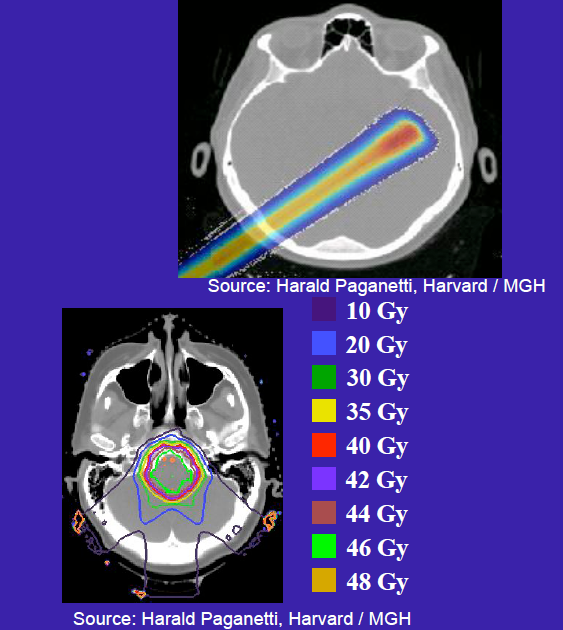
\includegraphics[height=7cm]{images/HarvardHadronTreatment.png}  
\caption{\label{fig:HarvardHadron} Example of Geant4 proton treatment simulation visualized.} 
\end{center}
\end{figure} 
Heavy-ion therapies have remained considerably less common and have remained on a more experimental level. Clinical trials were conducted at LBL inbetween 1977 and 1993 with $^{20}$Ne. At the end of 2008 the Particle Therapy Co-Operative  Group (PTCOG) estimated that more than 7000 heavy-ion treatments had been conducted at treatment facilities it monitors worldwide. Treatments based on $^{12}$C beams have been offered at NISR in Japan and in Germany at GSI~\cite{PTCOGstat}. Carbon beams is currently the most active and promising area of heavy-ion therapy research. 

The motivations for heavy-ion treatments as an alternative or complement to hadron treatments are considerable. Firstly carbon ions have the added advantage of higher ionisation-density at the end of their range, causing greater correlated damage to the DNA-structure of a single cancerous cell and therefore induces damage in a way that makes it less likely the cell is able to repair. In a 2008 article O.~Jäkel~\cite{ojakel} approximates the beam's increase in biological efficiency by a factor between 1.5 and 3 in comparison to proton treatment depending on the application. Secondly, Heavy-ions ions are less scattered in lateral directions which yields better dosage control in many applications. However, the tradeoff is that carbon-ions will fragment into smaller particles, yielding an unwanted ``tail`` to the energy-loss profile. One of the main motivations of the work is to study this ''tail'' for the ``worst case scenario'' of 400 MeV - an upper limit in medical applications.

A number of data-sets are available for carbon beams. This paper will be compare data to beam-measurments by E.~Haettner as a part of her master's thesis~\cite{ehaettner}  at the GSI facility in Darmstadt, Germany. This paper reproduces the experimental setup used by E.Haettner as a computer simulation model. The aim of this paper is to provide good reference data for the standardization work involved in hadron treatment. Furthermore, this paper evaluates the feasibility of the Geant4 models for such simulations by comparison to experimental data. This benchmarking is part of IAEA's INDC International Nuclear Data Committee and Heavy Charged-Particle Interaction Data For Radiotherapy project which compares different Monte-Carlo codes~\cite{SummaryReport}.\footnote{Bachelor's thesis produced in the framework of the Finnish CERN Summer Training 2009. Supervisors A.~Heikkinen and V.~Karimäki from Helsinki Institute of Physics and H.~Ehtamo of Helsinki University of Technology} %fixme footnote

%% Opinnäytteessä jokainen osa alkaa uudelta sivulta, joten clearpage
\clearpage
\section{Theory}

\subsection{Electromagnetic physics of Bragg-curve}
As charged particles penetrate tissue they interact with the tissue through elastic and inellastic collisions with the electrons and nuclei, eventually loosing all of their energy. The most typical interaction is that of inelastic collisions with electrons, contributing as much as 99\% of the total energy loss.

The beam's energy loss $dE/dx$ as a function of depth results is described by the Bragg curve (see fig). %fixme
 Theoretical estimates for this relation have existed since the first classical treatment by Bohr in 1913~\cite{bohr13}. The currently used quantum model was derived by Bethe and Bloch in 1953~\cite{bethebloch53}  and is commonly known as "Bethe's stopping power formula". The Bethe stopping power formula is considered a good model for most fast (E>...) %fixme larger than something
charged particles, with the exception of electrons.

\begin{equation}
 \frac{dE}{dx} = \frac{4 \pi}{m_e c^2} \cdot \frac{nZ^2}{\beta^2} \cdot \left(\frac{e^2}{4\pi\varepsilon_0}\right)^2 \cdot \left[\ln \left(\frac{2m_e c^2 \beta^2}{I \cdot (1-\beta^2)}\right) - \beta^2\right],
\label{bethebloch}
\end{equation}
where $\beta = v/c $, 
$v$ is the velocity of the particle,
$E$ is the 
energy of the particle,
$x$ is the 
distance travelled by the particle,
$c$ is the 
speed of light,
$Z$ is the 
particle charge,
$e$ is the 
charge of the electron,
$m_e$ is the 
rest mass of the electron,
$n$ is the 
electron density of the target and 
$I$  is the 
mean excitation potential of the target.


However, as the speed of the particle has decresed to the order of magnitude of the Bohr velocity the nuclear charge $Z$ will no longer remain constant and has to be aproximated by the effective charge, given by the Barkas formula. $$Z_{eff} = Z(1-e^{-125\beta_{P}Z})$$

In this theoretical model the form of the Bragg-peak can be visualized as the $1/v_{p}^2$ relation increases the energy-loss as speed decreases. However, the effective charge will decrease at an exponential rate, thus, converging the Bragg-curve.

Particles penetrating matter do not only deposit energy through inelastic electron collisions, they might as well be involved in nuclear reactions and fragmented. A common simple model for explaining this is called the abrasion-ablation model. In this model high energy projectiles can be described as particles that move on straight lines through the
target. From time to time a target nuclea lie on this line, thus causing a collision. Bullet
and target nucleons which overlap eachother in this model (see fig~\ref{fig:ablationabration}) are called participants. The remaining parts of the projectile and target nucleus are called spectators. The momentum of the spectators in the projectile and target are only slightly affected by the collision. The participant nucleons form an excited entity, ``a fireball'', which fragments into separate light ions or single nucleons.
The Wilson-model %fixme physics reference manual reference here
that also provided in Geant4 features a physics model more reminiscient to this approach. This kind of a model is however not directly comparable to the model used in this paper through INCL and ABLA.
\begin{figure}[h]
\begin{center}
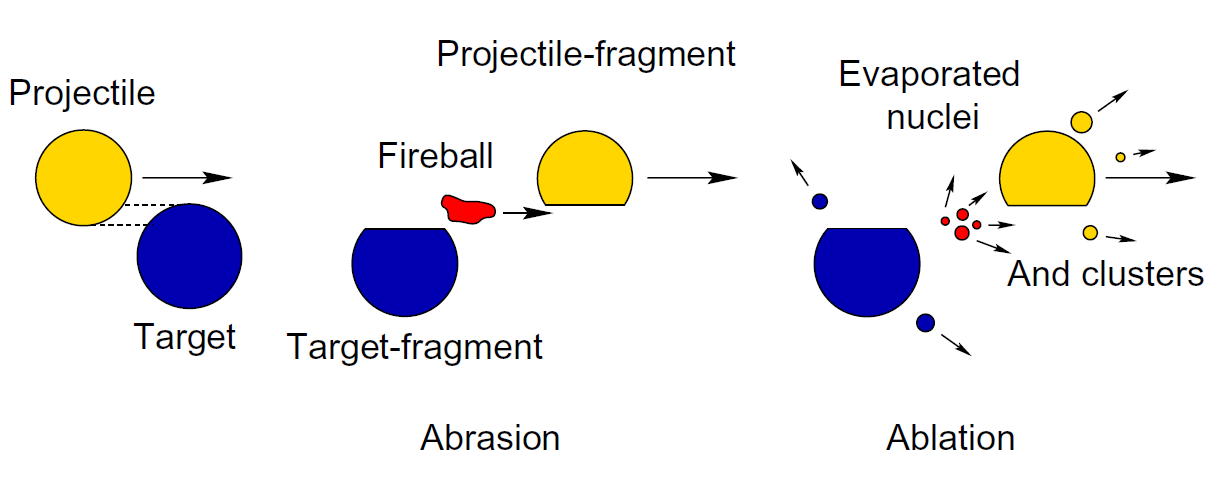
\includegraphics[width=0.8\textwidth]{images/ablationabration.png}  
\caption{Schematic description of the Wilson abration-ablation model in Geant4.}
 \label{fig:ablationabration}
 \end{center}
 \end{figure}



\subsection{Intranuclear cascade and fission/evaporation} %theory, no practical aspects

INCL4 is a Monte-Carlo type Intranuclear Cascade Model, whereas ABLA is the the complementing Monte-Carlo evaporation/fission model. In practice this means INCL is used to determine what happends just after the the projectile particle hits the target nucleus, while ABLA is used to determine what nuclear process is caused through the following excitation of the target due to the collision event. It is notable that the time-frame for evaporation and fission events are orders of magnitude greater compared to the events modelled by INCL.

\begin{figure} 
\begin{center}
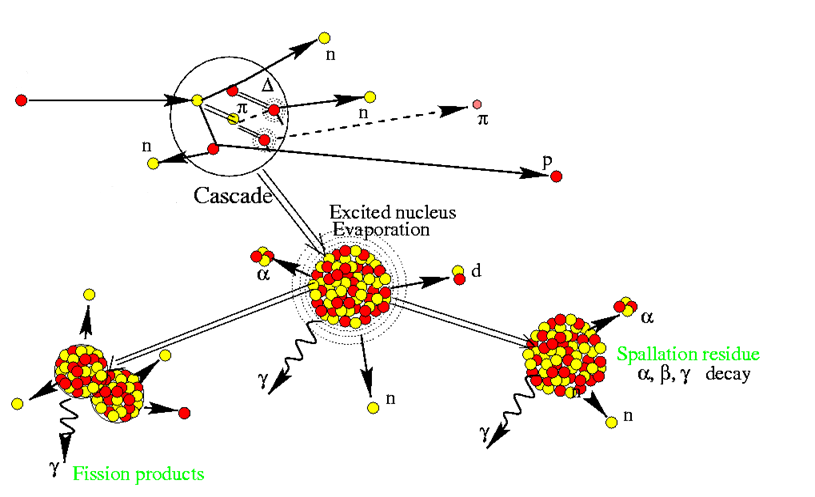
\includegraphics[width=0.8\textwidth]{images/inclScematic.png}  
\caption{\label{fig:inclschematic} Schematic diagram of INCL and ABLA models.}
 
 \end{center}
 \end{figure}


\subsubsection{INCL}

INCL is a implementation of the Liège INC model. It is designed for use in the 200MeV-2GeV region where standard cross-section libraries no longer are sufficient. Containing only few free parameters INCL has proven predictive power.

INCL is called into action when Geant4 selects from available model an inelastic collision will take place. INCL then takes as parameters the beam-particle and the target nucleus. It then proceeds to randomly pick what type of collision will happen by selecting the impact parameter between zero and the the target nucleus radius. The impact parameter is defined as the perpendicular distance between the velocity of the projectile and the center of the nucleus it is approaching.

In the Liège INC model particles move in straight deterministic trajectories, which makes upcoming collisions practical to predict in the INCL code.
 The nucleus in INCL is modelled as fermi-gas in a Woods-Saxon potential. %fixme woods-saxon
 The Woods-Saxon potential barrier gives a potential barrier that is smooth. Thus, in the INCL code the nucleons are randomly picked from a Woods-Saxon probability density distribution.

\begin{equation}
\rho(r) = \begin{cases}
\frac{\rho_{0}}{1+\exp({\frac{r-R_{0}}{a}})} & 0 < r < R_{max} \\
0 & \text{otherwise}
\end{cases}
\label{WoodsSaxon}
\end{equation}

If the energy of the bullet particle breaks the nucleus potential barrier and enters the nucleus several binary collisions between participating nucleons will take place, smaller particles may be emerge out from the nucleus. Spectator particles may move around the nucleus and bounce off its edges by reflection, however, they will not leave the nucleus.

The kinetics of the model are bound by the physical laws of conservation of baryon number, charge, energy, momentum and angular momentum and respect the Pauli blocking principle. Furthermore, pion-production is governed through the relation of $NN \rightleftharpoons N \Delta, \Delta \rightleftharpoons N\pi$ (with a stochastically determined mass for $\Delta$).

The major free parameter of the INCL code is the stopping-time; the time before thermal equilibrium can be assumed and thus the process handed over to the evaporation and fission phase. The INCL code has chosen the stopping time as a suitable function of the target nucleus size so that $$t_{stop} = f_{stop}t_{0}(\frac{A_T}{208})^{0.16},$$ where $f_{stop} = 1.0$. The stopping-time of INCL4 is considerably longer than for many models where discrete potential barriers are defined for the nucleus.

A further discussion of the theoretical basis of the Liège INC model and INCL code is available in references ~\cite{PhysRevC.66.044615,iia}.

\begin{figure}[ht]
\begin{center}
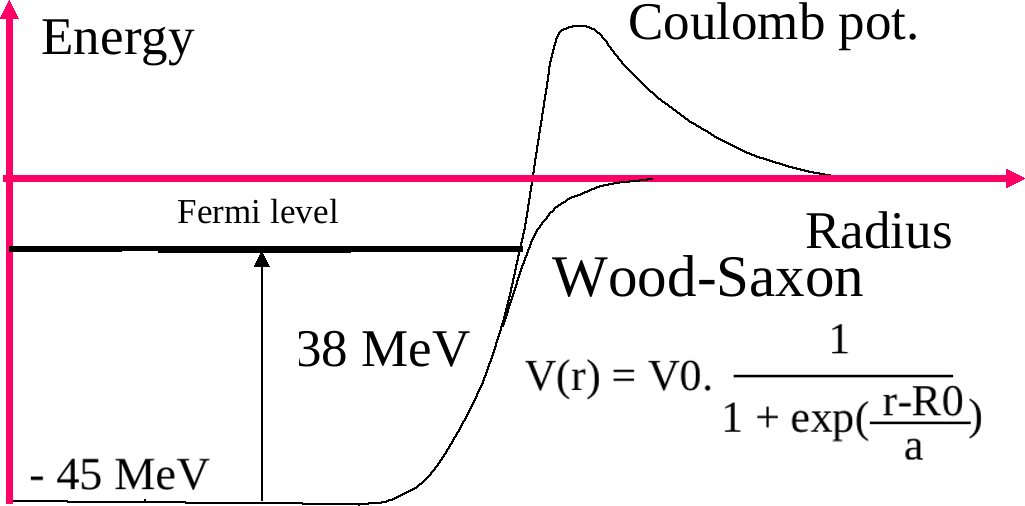
\includegraphics[width=0.3\textwidth]{images/inclPotential.png}  
\caption{\label{fig:inclpotential} Schematic of the potential model used by the INCL-model.}
 
 \end{center}
 \end{figure}


\subsubsection{ABLA}

The ABLA code has been developed at the GSI facility in Darmstadt, Germany. Its principal developers being K-H.~Schmidt and A.~Kelic. It is a Monte-Carlo code based on a data-set {\tt G4ABLADATA} distributed alongside the code. ABLA takes as input nucleus parameters, excitation energy, mass number, charge number and nucleus spin. It then calculates on the basis of this data the probabilities for different fission or evaporation events taking place according to statistical distributions obtained from experiments and phenomenology.

ABLA comes with two different fission models SimFis3 and SimFis18. These models are based on the proven PROFI-model also developed at GSI darmstadt. ABLA selects between competitive fission and evaporation processes as described in the flowchart~\ref{fig:ablatable}.

\begin{figure}[h] 
\begin{center}
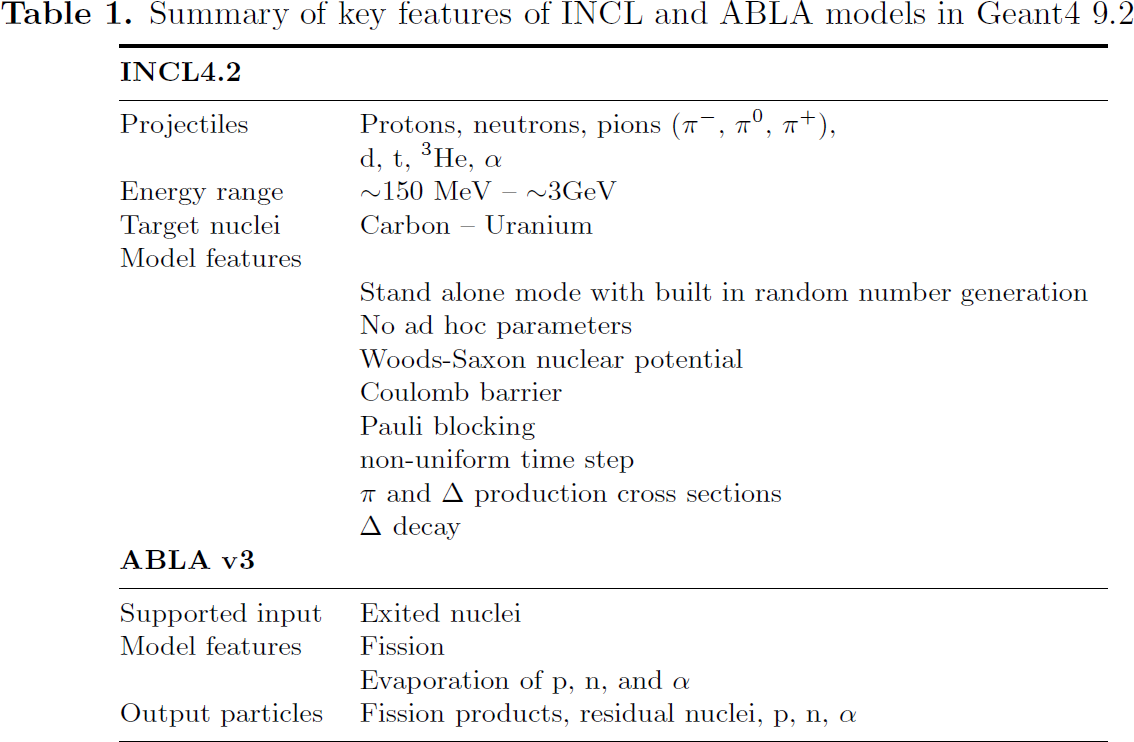
\includegraphics[width=1\textwidth]{images/inclSummary.png}  
\caption{\label{fig:inclpotential}}
 
 \end{center}
 \end{figure}

%fixme, add another picture with data

\begin{figure}[h] 
\begin{center}
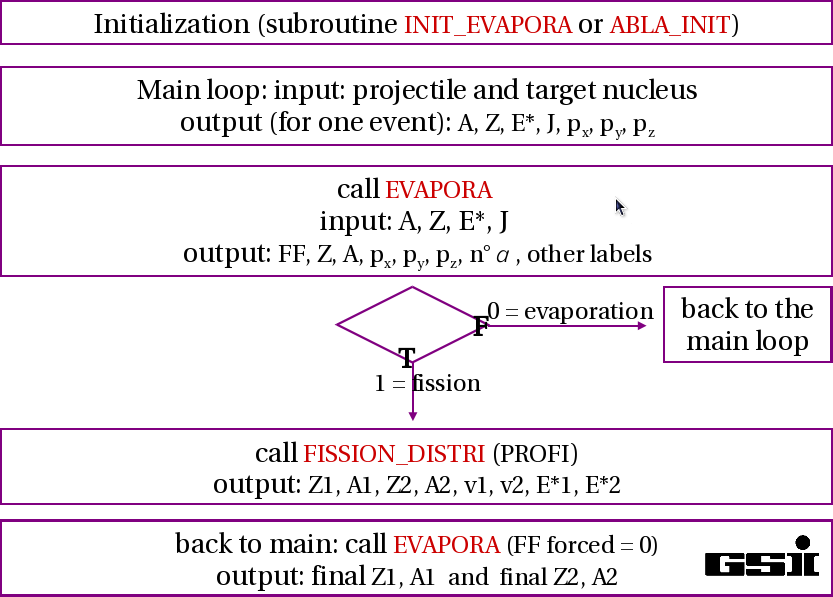
\includegraphics[width=0.6\textwidth]{images/AblaTable.png}[h]  
\caption{\label{fig:ablatable} General flow of ABLA submodels.}
 
 \end{center}
 \end{figure}
\begin{figure}[h] 
\begin{center}
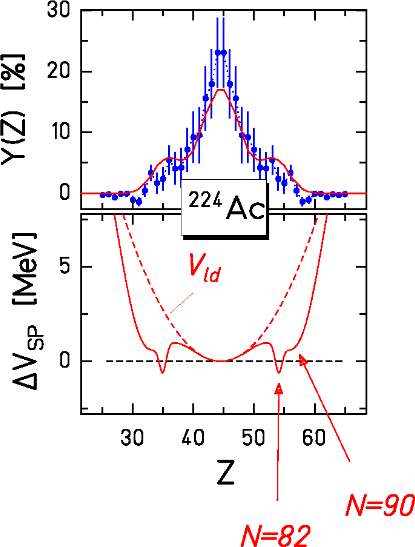
\includegraphics[width=0.3\textwidth]{images/AblaHumps.png}[h]  
\caption{\label{fig:ablahumps} ABLA symmetric (solid line) and antisymmetric (dashed line) fission plots.}
 
 \end{center}
 \end{figure}

A further discussion of the theoretical basis of the ABLA code is available in references ~\cite{ablatalk,iia}.
%fixme add another ABLAsource

\section{Simulation setup} %practical aspects of simulation
The simulation is to be performed with the latest versions of the INCL and ABLA code that is a part of the Geant4 suite.

\subsection{Characterization of the primary beam and experimental setup for the
IAEA benchmark}

Reference data for the measurements involved in this paper have been acquired from E. Haettner ~\cite{ehaettner}  Haettner performed these measurements at the GSI facility in Darmstadt, Germany. Haettner's experimental setup is presented below.

\begin{figure}[ht] 
\begin{center}
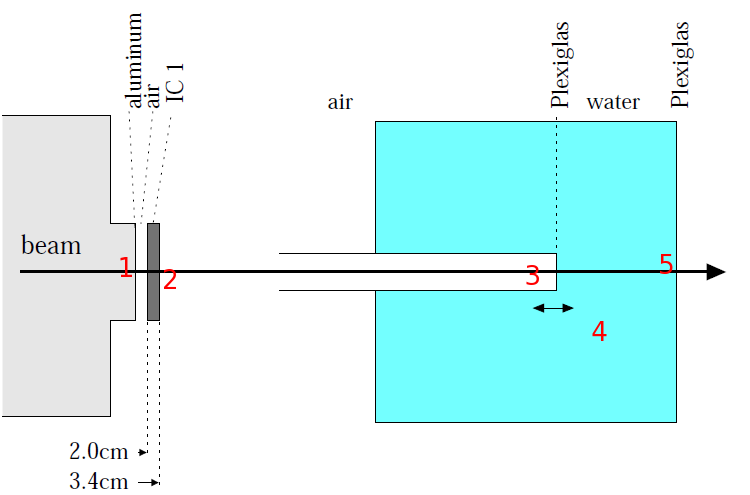
\includegraphics[width=0.9\textwidth]{images/haetnnersetup2.png}[h]  
\caption{\label{fig:haettnersetup} E.Haettner's experimental setup. The beam arrives at the experimental setup after traveling 10m from the last focuing magnets, thus it may be considered paralell at the time of entering the first detector.}
 \end{center}
 \end{figure}
\begin{figure}[ht] 
\begin{center}
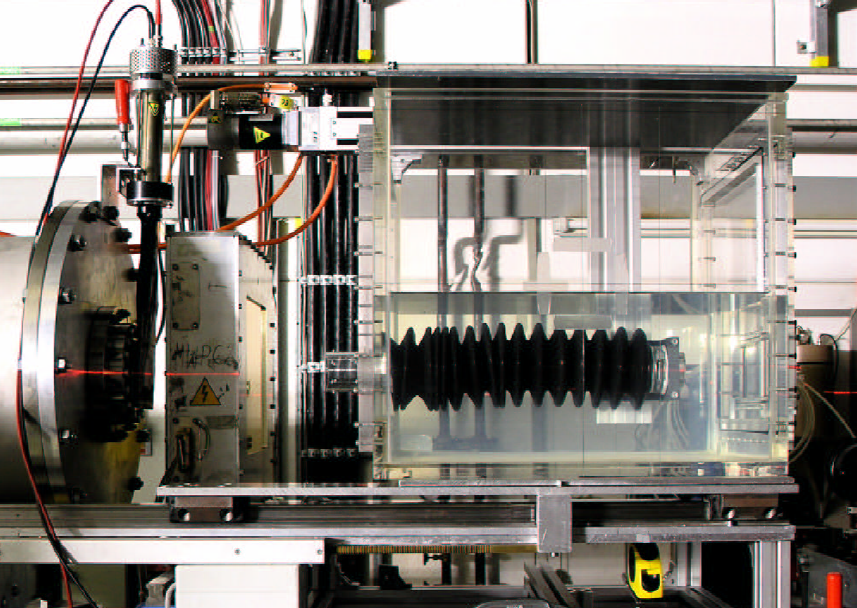
\includegraphics[width=0.9\textwidth]{images/haettnersetup.png}[h]  
\caption{\label{fig:haettnersetup2} E.Haettner's experimental setup. At the beam source the beam is assumed to be paralell and have an symmetric FWHM of 4mm. The beam first passes two detectors, then a water phantom and its cotnainer on both sides before reaching the last detector.}
 \end{center}
 \end{figure}

 \begin{table}[h]
\begin{tabular}{lllll} %fixme:
 & & & \textbf{200MeV} & \textbf{400 MeV} \\
1&Beam source window &\textbf{Aluminium}&0.1mm& 0.1mm\\
2&Ionization Chamber 1 &\textbf{Air-equivalent}&1.4cm& 1.4cm\\
3&Adjustable tube window &\textbf{Plexiglas}&2mm&2mm\\
4&Phantom &\textbf{Water}&0-30cm& 0-30cm\\
5&Container back-window &\textbf{Plexiglas}&2mm&2mm\\
6&Ionization chamber 2&\textbf{Air-equivalent}&3.7cm& 3.7cm\\
\end{tabular} 
\caption{\label{fig:SimSetup} The 1-d thicknesses of materials in the beam'a path. This presentation ignores effects induced by the true 3d-structure.}
\end{table}


\begin{figure}[ht] 
\begin{center}
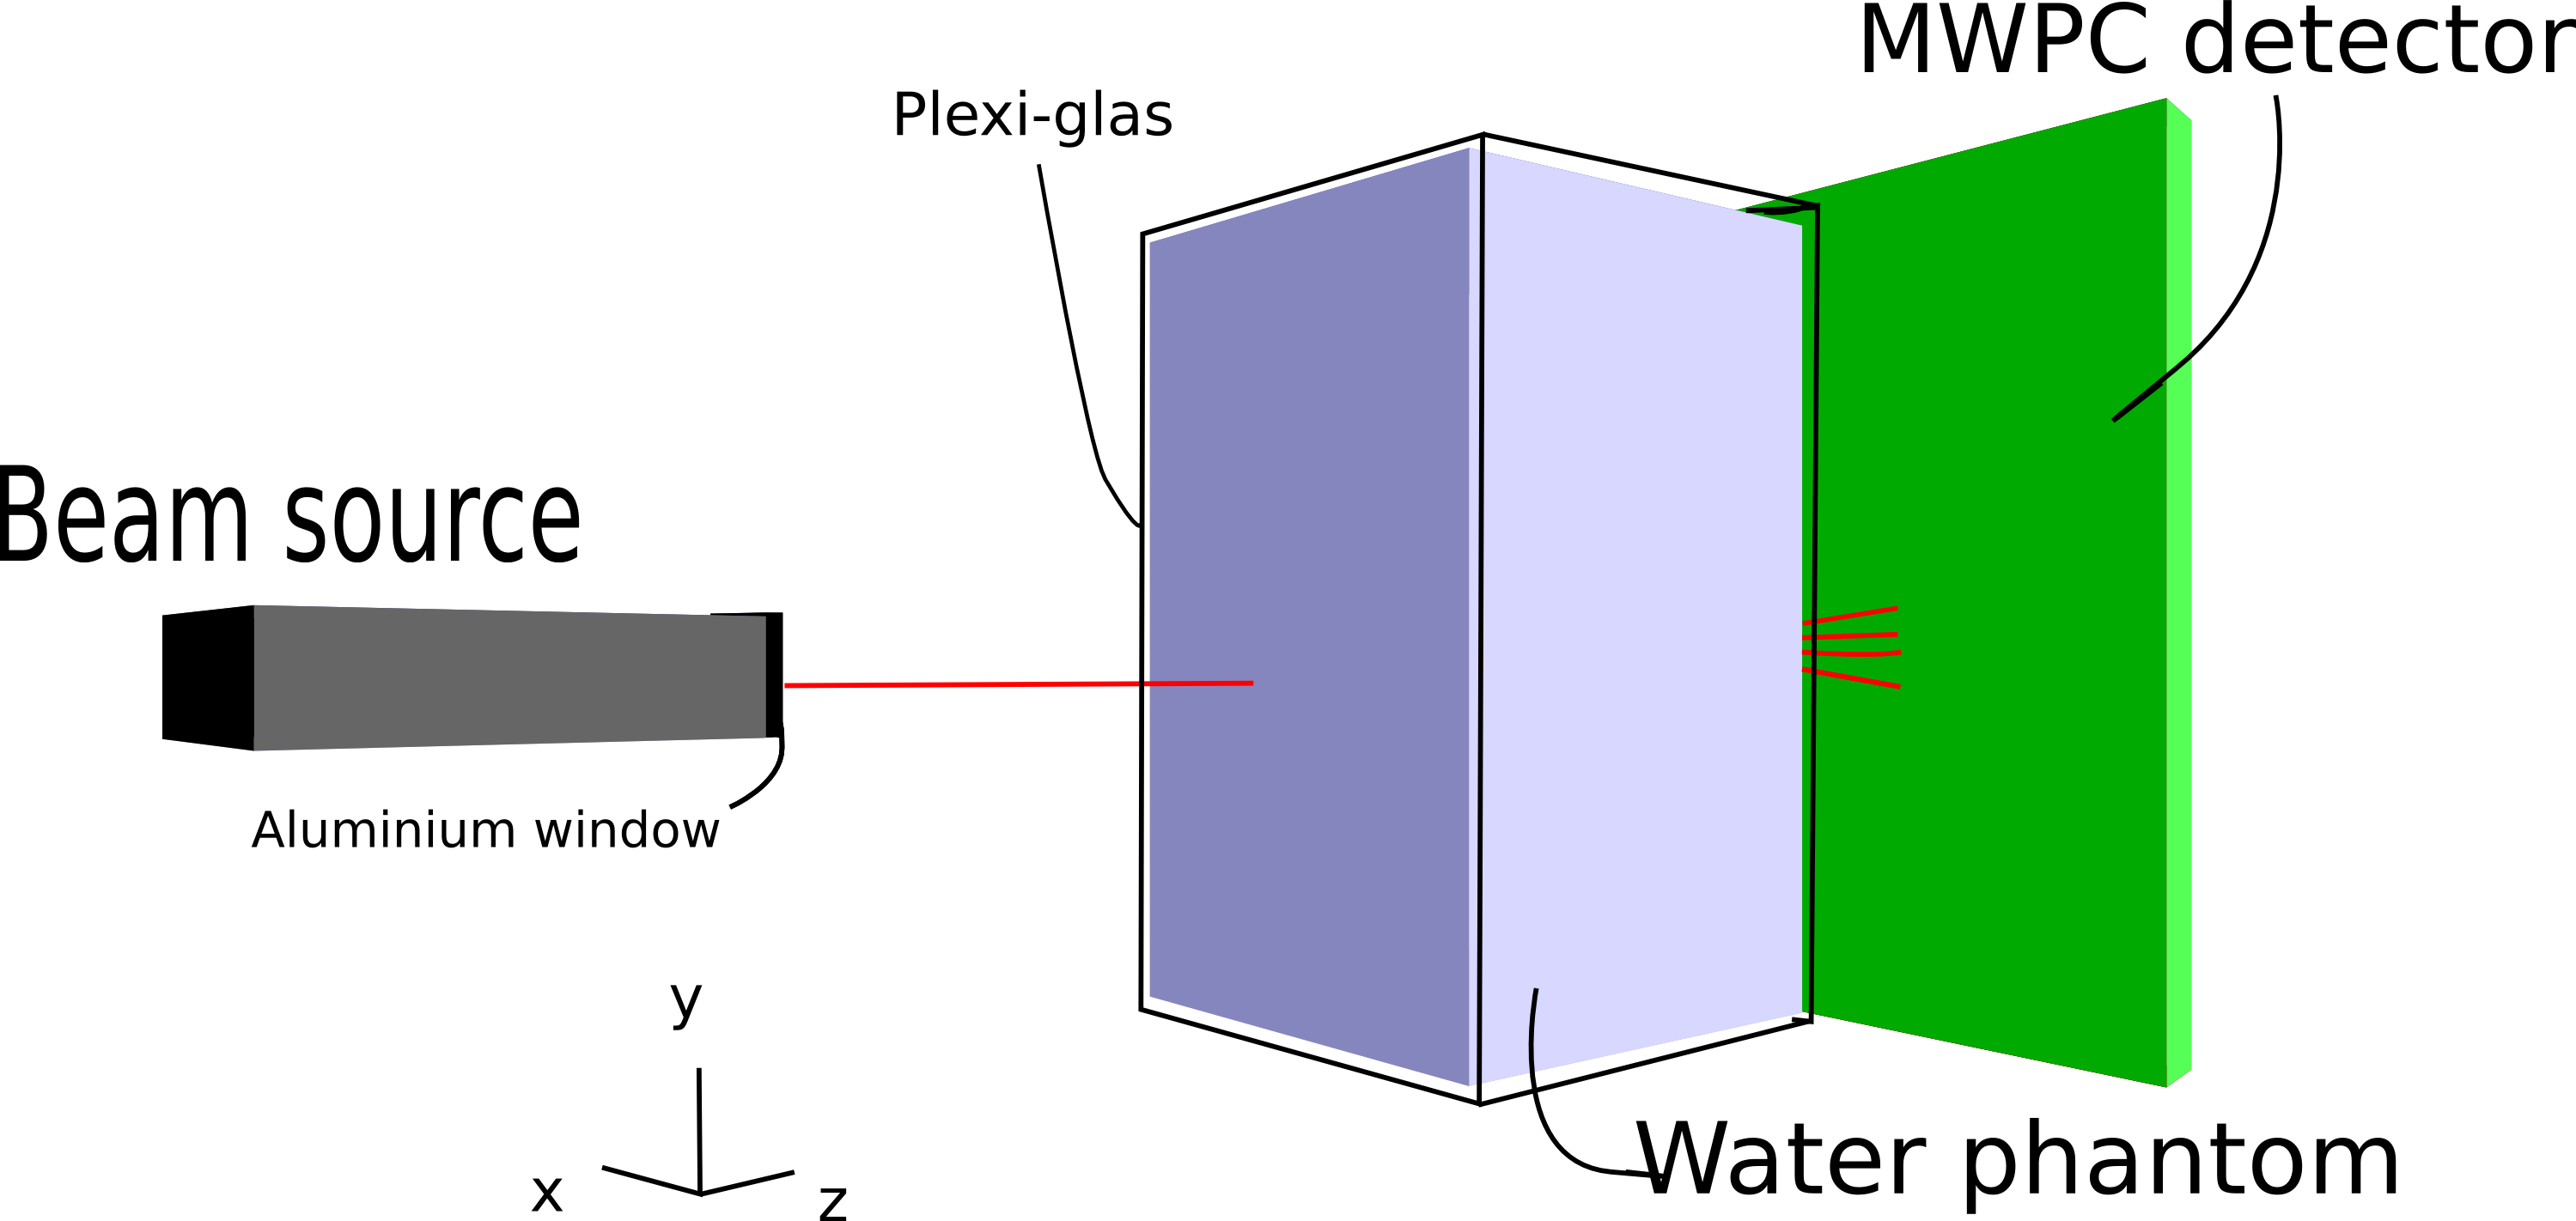
\includegraphics[width=0.9\textwidth]{images/SimSetup.png}[h]  
\caption{\label{fig:SimSetup} A simplified illustration of the simulation-setup. A beam passes an adjustable water-target and scatters. The scattering is measured by a simulated MWPC-detector.}
 \end{center}
 \end{figure}

%\begin{table}[h]
%\begin{tabular}{lllllll}
% & \textbf{200MeV} & & \textbf{400 MeV} & & \\
% &\textbf{thickness}&\textbf{mass / a.u.}&\textbf{WE}&\textbf{thickness}&\textbf{mass / a.u.}&\textbf{WE} \\
%\textbf{Aluminium}&0.1mm&0.027 $g/cm^2$& 0.027cm& 0.1mm&0.027 $g/cm^2$&0.027cm\\
%\textbf{Air and IC}&72cm &0.073 $g/cm^2$& 0.073cm& 91cm&0.109 $g/cm^2$&0.092cm\\
%\textbf{Plexiglas}&4mm&0.478 $g/cm^2$& 0.478cm& 4mm&0.476 $g/cm^2$&0.478cm\\
%\textbf{Water}&26.89cm&26.89 $g/cm^2$& 26.89cm& 8.04cm&8.04 $g/cm^2$&8.04cm\\
%\textbf{TOTAL}& &27.47 $g/cm^2$& 27.46 cm& &8.65 $g/cm^2$&8.64cm\\
%\end{tabular} 
%\caption{\label{fig:SimSetup} The 1-d thicknesses of materials in the beams path, ignoring effects induced by the true 3d-structure.}
%\end{table}


%\begin{center}
% \begin{table}[h]
%\begin{tabular}{llll} %fixme:
%& & \textbf{200MeV} & \textbf{400 MeV} \\
%Beam source window &\textbf{Aluminium}&0.1mm& 0.1mm\\
%Lab and IC's &\textbf{Air}&72cm& 91cm\\
%Water-container &\textbf{Plexiglas}&4mm& 4mm\\
%Phantom &\textbf{Water}&26.89cm& 8.04cm\\
%Beam source window &\textbf{Aluminium}&0.1mm& 0.1mm\\
%Lab and IC's &\textbf{Air}&72cm& 91cm\\
%Water-container &\textbf{Plexiglas}&4mm& 4mm\\
%Phantom &\textbf{Water}&26.89cm& 8.04cm\\
%\end{tabular} 
%\caption{\label{fig:SimSetup} The 1-d thicknesses of materials in the two beams' paths at the Bragg-peak. This presentation ignores %effects induced by the true 3d-structure.}
%\end{table}
%\end{center}



\begin{figure}[h] 
\begin{center}
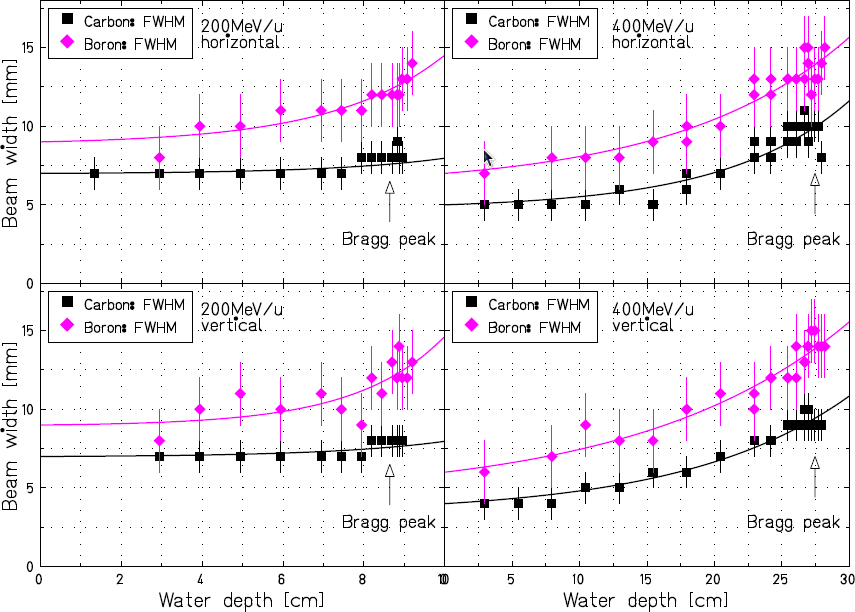
\includegraphics[width=0.9\textwidth]{images/haettner48.png}[h]  
\caption{\label{fig:haettner48} Haettner's experimental measurements of the relation between the depth in water and FWHM of different nucleons.}
 \end{center}
 \end{figure}

\subsubsection{Beam shape}

The beam is considered a pen-shaped beam. Haettner has performed several measurments to characterize the beam's accuracy. These results have to be reproduced in the simulated beamline correctly, and are thus evaluated in the thin-target experiment. Haettner produced the relation ~\ref{haettner48} for the depth in water and the FWHM of the beam. This relation has first to be verified in order to give further simulations credibility.

Haettner evaluates the accuracy of the beam's energy to be $\frac{\Delta E}{E}\approx5*10^{-3}$, meaning that the energy distribution of the beam is very narrow. However, this error was simulated with a gaussian distribution with the standard deviation 1 meV/u and 2MeV/u for the 200 respectively 400 MeV Beams.

In this simulation the beam is reproduced at the beam source (see ~\ref{fig:SimSetup}) as measured by Haettner with no phantom and zero distance from start detector to the last detector. The beam is measured right after the beam-source window. The beam-source itself is assumed to produce a paralell beam. The first source of scattering the beam is the aluminium window of the beam-source, but as this measurement is made right after the window it can be used to characterize the paralell beams width. However inspecting further measurements at 1 and 3 meters show the effects of scattering in the aluminium, detectors and air as a broadening beam. The scattering of the beam is considerably different depending on the energy of the beam.

However the beam width is similar at the time of entering the experiment. The beam will therefore in the simulation at its origin have an FWHM of 4mm as per E.Haettner 4.7. A gaussian FWHM of 4mm is equivalent to a standard deviation of 9.42mm according to the relation $\mathrm{FWHM} =   2 \sqrt{2 \ln 2 } \; \sigma \approx 2.35482 \; \sigma$. %perhaps the mwpc should be accounted for or simulated?

E.Haettner proceeds to analyze the scattering of the beam with variable water thicknesses. When no water is used the paralell beam is scattered solely by the aluminium and air along its path. This experiment can be reproduced as a thin-target simulation where the beam passes through 0.1 mm of aluminium before its scattering is measured at various distances. This was done by simulating Haettner's MWPC detector with a similar size body with no physical density but with the logical function to register particles upon entry by their type and displacement in on the x and y axises. After the particles have been registered upon entry in the volume they are removed from the simulation.

\subsubsection{Beam attenuation}

%In order to calculate the Bragg Curve of the beam the previous experiment a set-length water-phantom of 40 cm was placed in the path of %the beam as illustrated. The amount of water was approximated on the basis of E.Haettner's work so that the entire bragg-curve and a %considerable part of the fragment-tail would be visible. This water-phantom was divided into 1x1x400 voxels. This in effect means the %water-phantom was presented as 400 logical perpendicularily to the beam placed ``slices''. The bragg-peak is calculated by saving the %energy-deposits in every slice at all times. Thus a histogram presenting a characteristic bragg-curve appears.

In order to calculate the Bragg-curve available in the data-set the thickness of the water-phantom was varied. The MWPC detector was then augmented with the ability to register the energy of the incoming particles. Repeating this simulation for a number of water-depths gives the characteristic Bragg curve with its fragment-tail.






%\begin{comment}
%Koska lupasin koordinoida speksien määärittelyn.
%voisit Gillis tehdä raporttiisi seuraavaksi alaluvun :
%'Characterization of the primary beam and experimental setup for the
%IAEA benchmark'
%Ennen kun rupeat rakentamaan Geant4 simulaatiota  voisit siis kerätä
%Emman työstä
%kaikki vaadittavat tiedot (etäisyydet, materiaalit, dimensiot, beamin
%tiedot) tähän lukuun.
%Tämän tekstin tulisi olla itsenäinen osa opinnäytetyötä jotta sen voi
%kätevästi jakaa muiden Monte-Carlo koodien edustajlle.
%(Näppärä taulukko ja kuva kuten gradussa selventävät asiaa.) Tekstin
%pohjalta pitää pystyä luomaan
%yksikäsitteisesti oikeanlainen Monte-Carlo koe jonka tuloksia sitten
%verrataan Emman mittauksiin.

%doc/talk/images/inclSummary.png
%images/haettnersetup.png
%\end{comment}

\begin{itemize}
\item Experiment data from GSI
\item target description
\item Characterization and simulation of the beam (will be ignored, gaussian shape half-width fullheight HWFH assumed narrow pen beam - randomly pick in a small gaussian beam error perhaps - g4uniformrand-gaussian or check )
\item Simulation of detectors
\item Implementation details
\end{itemize}

\subsection{Improving usability through messenger macro commands}
The first action task taken in this work was to implement means of saving analysis files with a user-defined name.

So as aen example the user can give a command according to the following syntax.
\scriptsize
\begin{verbatim}
/analysis/setFileName <user-defined name>.root
\end{verbatim}
\normalsize

The implementation was done by creating an analysismessenger inheriting functionality from \textit{G4UImessenger}. An object of the type \textit{HadrontehrapyAnalysisMessenger} was created in the \textit{AnalysisManager}.


\scriptsize
\begin{verbatim}
class HadrontherapyAnalysisFileMessenger: public G4UImessenger
{
  public:
    HadrontherapyAnalysisFileMessenger(HadrontherapyAnalysisManager*);
   ~HadrontherapyAnalysisFileMessenger();
    
    void SetNewValue(G4UIcommand*, G4String);
    
  private:
    HadrontherapyAnalysisManager* AnalysisManager;
\end{verbatim}
\normalsize
\begin{figure}[h] 
\begin{center}
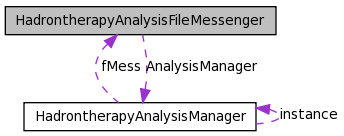
\includegraphics[width=0.3\textwidth]{images/setFileNameMessenger_1.png}  
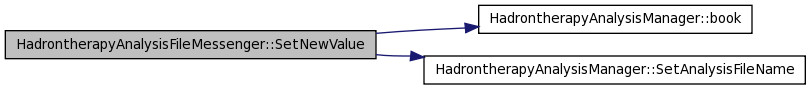
\includegraphics[width=0.7\textwidth]{images/setFileNameMessenger_2.png}  
\caption{\label{fig:messengerUML} UML diagrams for messen ger class}
 
 \end{center}
 \end{figure}

\section{Results and comparison to GSI data}
\begin{itemize}
\item comparison (Haettner 5.4.1)
\item energy distribution of fragments
\end{itemize}

\section{Conclusion}
\begin{itemize}
\item Raflaava yhteenveto
\end{itemize}

\section{Appendices}
\begin{itemize}
\item code examples
\item runtime log
\end{itemize}





\bibliographystyle{plain} \bibliography{refs.bib} 

%%%%% Liitteet 
%\appendix 

%\clearpage
%\addcontentsline{toc}{section}{Liite A}
%\section*{Liite A \label{LiiteA}}

%% Liitteiden kaavat, taulukot ja kuvat numeroidaan omana kokonaisuutenaan
%\renewcommand{\theequation}{A\arabic{equation}}
%\setcounter{equation}{0}  
%\renewcommand{\thefigure}{A\arabic{figure}}
%\setcounter{figure}{0}
%\renewcommand{\thetable}{A\arabic{table}}
%\setcounter{table}{0}


\end{document}



